\documentclass[11pt, norsk]{article}
%\usepackage[latin1]{inputenc}
\usepackage[T1]{fontenc}
\usepackage[utf8]{inputenc}
\usepackage[norsk]{babel}   % S P R A A K


\usepackage{graphicx}    % postscript graphics
\usepackage{amssymb, amsmath, amsthm, amssymb} % symboler, osv
\usepackage{mathrsfs}
\usepackage{url}
\usepackage{thmtools}
\usepackage{enumerate}  % lister $  
\usepackage{float}
\usepackage{tikz}
\usetikzlibrary{calc}
\usetikzlibrary{intersections}
\usepackage{tikz-3dplot}
\usepackage{subcaption}
\usepackage[all]{xy}   % for comm.diagram
\usepackage{wrapfig} % for float right
\usepackage{hyperref}
\usepackage{mystyle} % stilfilen      


\begin{document}
\title{Oppgaver MAT2500}
\author{Fredrik Meyer}
\maketitle 

\begin{oppg}
La $P=(1:0:0)$, $Q=(1:1:0)$, $R=(1:0:1)$ og $S=(1:1:1)$ være punkter i $\PP^2_\R$. Regn ut snittet av $\ol{PQ}$ og $\ol{RS}$.
\end{oppg}
\begin{losn}
Vi finner først ligningen for linjen $\ol{PQ}$. Den mekaniske måten er å skrive ut determinanten
$$
\begin{vmatrix}
 x_0 & x_1 & x_2 \\
 1 & 0 & 0 \\
1 & 1 & 0
\end{vmatrix} = 0
$$
Vi får $x_2=0$, som vi kunne gjettet oss til ved å se på punktene (...).

Tilsvarende finner vi at $\ol{RS}$ er gitt ved $x_0-x_2=0$ (dette er riktig fordi ligningen $x_0-x_2=0$ definerer en projektiv linje, og $R,S$ begge ligger på denne linjen).

Dermed er snittet deres gitt av ligningssystemet $x_2=0, x_0-x_2=0$. Altså $x_0=x_2=0$. Med andre er snittet lik punktet $(0:1:0)$. 
\end{losn}

\begin{oppg}
Lag et projektiv plan med 13 punkter og 13 linjer.
\end{oppg}

\begin{losn}
Dette er vanskeligere enn det høres ut som. Mange har kanskje sett Fano-planet med syv elementer. Se Figur 1.
\begin{figure}
 \centering
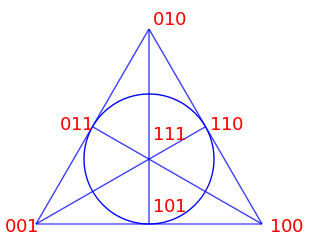
\includegraphics[width=90mm]{fanoplane}
  \caption{Fano-planet.}
\end{figure}  
Legg merke til at koordinatene. Legger du sammen to punkter på sammme linje får du det tredje punktet, så dette er en spesielt pen framstilling.

Det finnes også et projektiv plan med $13$ elementer. Én mulighet er å tegne det på samme måte som Fano-planet, altså som en trekant med homogene koordinater og standardkoordinatene $(1:0:0),(0:1:0)$ og $(0:0:1)$ på hjørnene. Dessverre blir ikke dette bildet på langt nær så pent som Fano-planet. Se Figur 2 og 3 for to muligheter.
\begin{figure}
  \centering
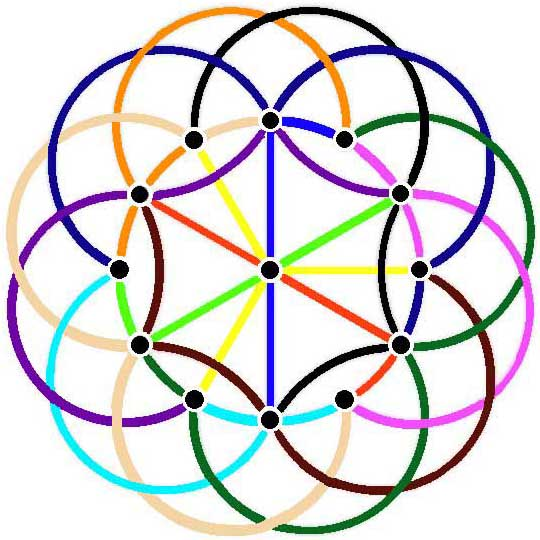
\includegraphics[width=90mm]{projplane13.jpg}
  \caption{En veldig symmetrisk framstilling av $\PP^2_{\mathbb F_3}$.}
\end{figure}
\begin{figure}
\centering
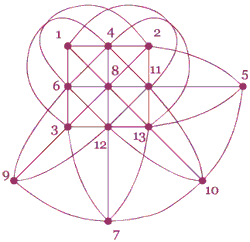
\includegraphics[width=90mm]{proj132}
  \caption{En annen, kanskje mer oversiktlig framstilling.}
\end{figure}
Vi ser at Figur 2 er mer symmetrisk, men Figur 3 er mer oversiktlig. 
\end{losn}

\end{document}
